\chapter{Literature Review}
\label{ch:review}

This chapter reviews four bodies of evidence that motivate the study design:
the distinction between statistical and machine-learning models
(Section~\ref{sec:false_dichotomy}), variability in sepsis labels and their
dependence on clinical action (Sections~\ref{sec:label_object}
and~\ref{sec:label_action}), internal, temporal and external validation and the
gap between discrimination and clinical utility
(Sections~\ref{sec:generalisation} and~\ref{sec:auroc_illusion}), and
methodological choices in dynamic survival modelling
(Section~\ref{sec:survival_dispute}). It then considers rule-based comparators,
subgroup validity and interpretability
(Sections~\ref{sec:comparator_choice}--\ref{sec:interpretability_survives}),
and Section~\ref{sec:design_warrant} summarises the evidence behind each design
decision taken in Chapter~\ref{ch:methodology}.


\section{Search Strategy}
\label{sec:search_strategy}

The literature search targeted published work on real-time sepsis prediction,
with particular attention to label sensitivity, validation methodology,
evaluation metrics and subgroup validity. Table~\ref{tab:search_strategy}
documents the protocol. A companion review, \textit{Statistical and
Machine-Learning Approaches to Real-Time Sepsis Onset Prediction on MIMIC-IV},
covers the full corpus of 50 sources, including several of contextual
relevance only; this chapter engages with the sources that bear on the study's
design decisions.

\paragraph{Type of review.} This is a \textbf{structured narrative review, not
a PRISMA-conformant systematic review}. Searches followed a documented protocol
and every included source was verified against a primary record, but a
complete deduplicated search yield was not screened by title and abstract, and
no second reviewer screened independently. The search covers in depth the
methodological literature that constrains this study, but not the MIMIC-IV
sepsis corpus exhaustively. The novelty claims in Section~\ref{sec:contrib} are
bounded accordingly, and a systematic review could identify a prior study
combining the analyses in contribution C1 or C5. Throughout this thesis, a
statement that no study was identified refers to this search.

{\small
\begin{longtable}{p{3.2cm}p{9.5cm}}
    \caption{Literature search strategy, supporting the novelty claims for
    contributions C1 and C5 (Section~\ref{sec:contrib}).}\label{tab:search_strategy}\\
    \toprule
    \textbf{Element} & \textbf{Detail} \\
    \midrule
    \endfirsthead
    \toprule
    \textbf{Element} & \textbf{Detail} \\
    \midrule
    \endhead
    \bottomrule
    \endfoot

        Databases searched &
        PubMed/MEDLINE, Embase, Scopus, Web of Science, IEEE Xplore,
        ACM Digital Library, Google Scholar, Cochrane Library,
        ScienceDirect, SpringerLink, Wiley Online Library, Nature
        Portfolio, JAMA Network, BMJ Journals, arXiv/medRxiv \\
        \addlinespace
        Searches executed &
        35 structured searches across the domains listed under ``Search
        terms'' \\
        \addlinespace
        Date range &
        Primary sepsis-prediction literature: January 2015 -- July 2026.
        Methodological and definitional foundations (e.g.\ pooled logistic
        regression, decision-curve analysis) were searched without a date
        limit, and the earliest source retained dates from 1990 \\
        \addlinespace
        Search terms &
        \texttt{(sepsis OR ``sepsis prediction'' OR ``sepsis detection'') AND
            (MIMIC OR ``critical care'' OR ``intensive care'')} combined with each
        of: \texttt{``label definition''}, \texttt{``label sensitivity''},
        \texttt{``onset definition''}, \texttt{``utility score''},
        \texttt{``clinical utility''}, \texttt{``fairness'' OR ``equity'' OR
        ``disparity'' OR ``bias''}, \texttt{``subgroup analysis''},
        \texttt{``competing risks'' OR ``discrete-time survival''} \\
        \addlinespace
        Inclusion criteria &
        (1)~Peer-reviewed journal article, conference paper, or preprint on a
        recognised server (arXiv, medRxiv);
        (2)~Develops or evaluates a real-time (hourly or sub-hourly) sepsis
        prediction model;
        (3)~Uses EHR data from an ICU population;
        (4)~Reports at least one quantitative performance metric \\
        \addlinespace
        Exclusion criteria &
        (1)~Non-English language;
        (2)~Editorials, commentaries, or letters without original results;
        (3)~Models for sepsis severity staging or mortality only (not onset
        prediction);
        (4)~Studies on paediatric or neonatal populations exclusively \\
        \addlinespace
        Verification standard &
        Every included source was checked against a publisher record, PubMed or
        PMC record, or institutional repository entry, with journal, volume,
        year and DOI confirmed. Every numerical claim attributed to a source
        was located in that source's own abstract, results text or
        publisher-hosted record, never inferred from a secondary citation \\
        \addlinespace
        Total included &
        50 sources in the companion review: 46 identified and verified through
        the searches above, and 4 retained from an earlier base review of 19
        sources. 45 are cited in this thesis \\
        \addlinespace
        Excluded at verification &
        4 items encountered in secondary citation lists could not be verified
        to the standard above and were excluded; 1 further item is retained in
        the companion review with an explicit note of incomplete metadata and
        is not cited in this thesis \\
\end{longtable}
}

Figure~\ref{fig:prisma} summarises the identification, verification and
inclusion process, following the reporting logic of PRISMA 2020
\cite{page2021prisma}.

\begin{figure}[H]
\centering
\adjustbox{max width=\textwidth}{%
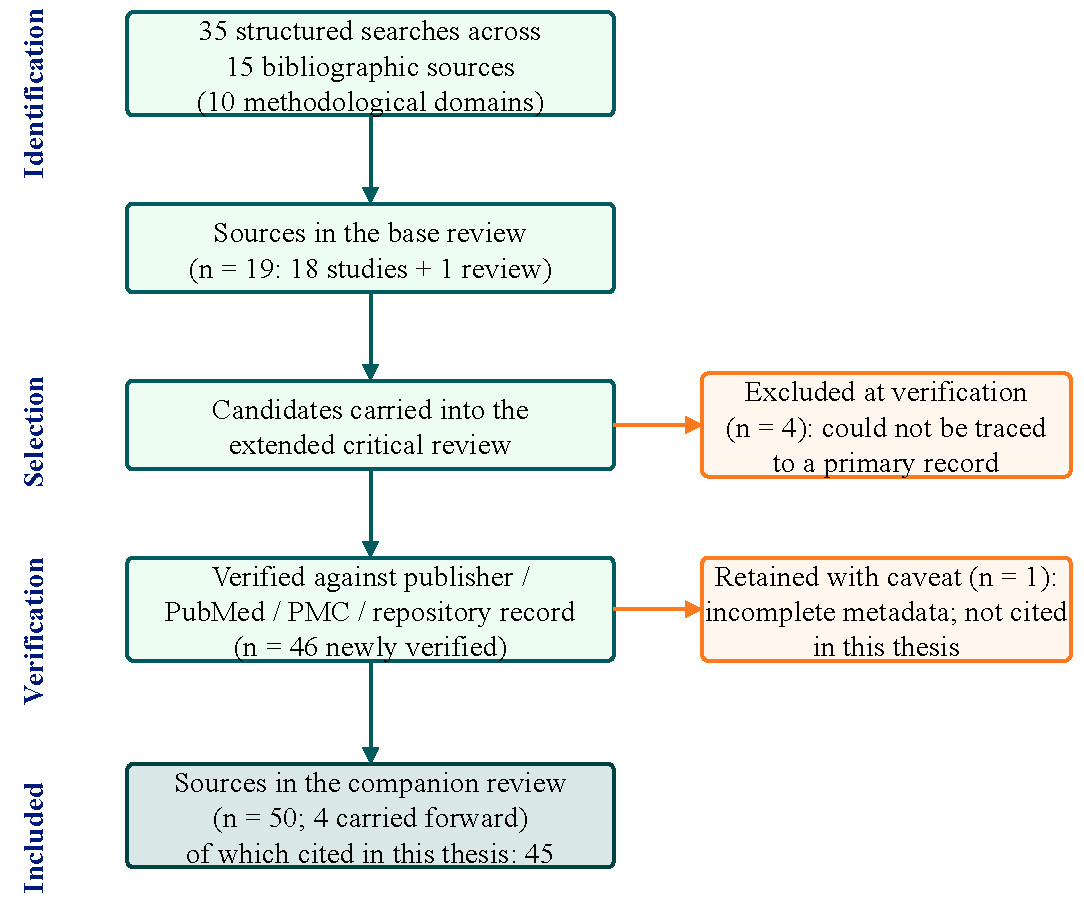
\includegraphics[width=0.82\textwidth]{figures-img/fig2.1_prisma.pdf}}
\caption{Search, verification and inclusion flow, following the reporting
  logic of PRISMA 2020 \cite{page2021prisma}. It is not a PRISMA flow diagram:
  no title-and-abstract screening of a full deduplicated yield was performed,
  and no second reviewer screened.}
\label{fig:prisma}
\end{figure}

\paragraph{Novelty claims supported by the search.}
Two contributions rest on search-based evidence. Each concerns a
\emph{combination} of analyses with clear individual precedent; the search
identified no study performing them together.

\begin{enumerate}
    \item \textbf{C1 (Label variation under a dynamic survival model).} Label
    sensitivity is well established \cite{johnson2018comparative,
    cohen2024subtle, dutta2026performance}, and the last two studies are
    direct precedents for this one. Cohen et al.\ include a survival model
    among the families they compare, so the survival setting is not new
    either. The search identified no study applying three or more Sepsis-3
    operationalisations to a \emph{discrete-time competing-risks} model on
    MIMIC-IV and reporting the label spread with an interval alongside the
    model-class spread on the same test rows.

    \item \textbf{C5 (Performance disparity and label sensitivity across the
    same subgroups).} Wang, Li, Naidech and Luo \cite{wang2022equity} report
    both subgroup performance disparity and subgroup variation in who is
    labelled septic, but for mortality prediction rather than sepsis onset
    (Section~\ref{sec:equity_lit}), so their study does not provide a direct
    precedent for an onset model's subgroup performance. Studies of label
    sensitivity for onset prediction (Cohen et al., Dutta et al.) do not
    stratify by demographic subgroup. The contribution lies in evaluating
    subgroup discrimination and subgroup label sensitivity on the same strata
    of one onset-prediction cohort under a common multiplicity procedure.
\end{enumerate}

\paragraph{Scope of the clinical-utility evidence.}
Wang et al.\ \cite{wang2025srpm} reviewed 91 real-time sepsis prediction
models. Only a minority reported the PhysioNet Utility Score
\cite{reyna2020utility} or an equivalent net-benefit metric; the Utility Score
rewards early true alerts, penalises late alerts and false alarms, and is
normalised so that issuing no alerts scores zero. The majority reported only
AUROC, AUPRC or both. Among the models with a utility or net-benefit metric,
the median external Utility Score was $-0.164$, indicating net harm. For
models reporting only AUROC, clinical utility could not be assessed, and no
claim about their utility is made here.

\paragraph{Key concepts.} \textbf{MIMIC-IV} (Medical Information Mart for
Intensive Care, version IV) is a freely available, de-identified database of
approximately 74,000 ICU admissions at Beth Israel Deaconess Medical Center,
Boston, covering 2008--2019 \cite{johnson2023mimiciv}. \textbf{Sepsis-3} is the
current international consensus definition of sepsis as life-threatening organ
dysfunction caused by a dysregulated host response to infection, operationalised
through suspected infection (an antibiotic order plus a culture draw) together
with a rise of at least 2 points in the Sequential Organ Failure Assessment
(SOFA) score \cite{singer2016sepsis3}.

\subsection*{Review Questions}

Four questions structure the review:

\begin{enumerate}
    \item[\textbf{RQ1.}] How much does the choice of sepsis label definition
    affect model performance, and is this effect comparable in magnitude to
    the choice of model architecture? (Sections~\ref{sec:false_dichotomy}
    and~\ref{sec:label_object})
    \item[\textbf{RQ2.}] Which methodological choices (validation strategy,
    metric selection, treatment-time leakage) most affect reported performance
    in the sepsis prediction literature? (Sections~\ref{sec:label_action}
    to~\ref{sec:auroc_illusion})
    \item[\textbf{RQ3.}] What statistical framework is appropriate for
    modelling hourly ICU event data when proportional-hazards and
    independent-censoring assumptions may not hold?
    (Section~\ref{sec:survival_dispute})
    \item[\textbf{RQ4.}] Does the existing equity literature on sepsis
    prediction account for label-level variation across demographic subgroups,
    or only model-level variation? (Section~\ref{sec:equity_lit})
\end{enumerate}


\section{Reconsidering the Statistical versus Machine-Learning Distinction}
\label{sec:false_dichotomy}

Reviews of this literature conventionally divide it into a statistical
tradition and a machine-learning tradition, and the distinction is often
associated with interpretability on one side and predictive performance on the
other. For this study, a distinction based on temporal modelling assumptions
is more informative.

Several boundary cases illustrate this. The Artificial Intelligence Sepsis
Expert \cite{nemati2018aise}, commonly classified as machine learning, uses a
modified Weibull--Cox proportional-hazards formulation. TREWScore
\cite{henry2015trewscore}, a Cox model and a commonly used statistical
benchmark for this task, is often described in the machine-learning literature
as an early machine-learning early-warning system, and its commercial
successor is marketed as one \cite{adams2022trews}. Cohen et al.\
\cite{cohen2024subtle} compare tree-based, deep-learning and survival models
within a single frame, and TRIPOD+AI \cite{collins2024tripodai} covers
``regression or machine learning'' under one checklist, having concluded that
the reporting failures it addresses are common to both.

A more informative distinction separates models by what they assume about
time.

\begin{itemize}
    \item \textbf{Static models} take a snapshot (baseline, day one, or the
    worst value in the first 24 hours) and issue one prediction. Much of the
    MIMIC-IV statistical corpus sits here: a candidate biomarker or composite
    index is regressed on mortality through a largely standard pipeline of
    variable selection, Cox and logistic regression, splines, a nomogram, and
    ROC, calibration and decision curves. These are \emph{prognostic}
    instruments and cannot perform real-time onset detection.
    \item \textbf{Dynamic models} consume a stream and update a risk estimate as
    it arrives. TREWScore, the Artificial Intelligence Sepsis Expert, the
    PhysioNet Challenge entries \cite{reyna2020utility}, Moor et al.'s deep
    temporal model \cite{moor2023review}, and landmark and joint models all sit
    here. Whether the update rule is a partial likelihood, a recurrent network
    or a boosted hazard is secondary for this distinction.
\end{itemize}

This framing also corrects the claim that statistical methods have neglected
onset prediction. Henry et al.\ \cite{henry2015trewscore} fitted a Cox model
for septic-shock onset on MIMIC-II; Fagerstr{\"o}m et al.\
\cite{fagerstrom2019lisep} fitted one on MIMIC-III with Henry et al.'s inputs
and target as the baseline for an LSTM; and Cohen et al.'s survival arm does so
on MIMIC-III again. The search identified no MIMIC-IV study combining dynamic
onset modelling, explicit assumption testing, label-sensitivity analysis and
temporal validation.

The evidence on model class is similarly scoped. Christodoulou et al.\
\cite{christodoulou2019cox}, reviewing 71 studies, found no performance
advantage for machine learning over logistic regression in clinical
prediction, and observed potential bias in the validation procedures of 68\%
of them; their evidence concerns binary outcomes on tabular data. For temporal
early warning, Fagerstr{\"o}m et al.\ report their deep model detecting
patients up to 20 hours earlier than the Cox model at comparable sensitivity
and specificity. Equivalence is therefore supported for static risk
stratification but remains contested for temporal early warning. H6 tests this
narrower comparison with the data, the label, the validation split and the
evaluation held fixed.

The literature has two further implications for design. Moor et al.'s
systematic review \cite{moor2021review} identifies low comparability and
reproducibility as the field's principal defect, and highlights case--control
matching as a specific risk: when a control patient's reference time is chosen
near discharge while a case is aligned near onset, the two are easily
separated and apparent performance is inflated. Fleuren et al.\
\cite{fleuren2020ml}, in a meta-analysis of diagnostic test accuracy,
attribute the between-study heterogeneity that prevented pooling to
methodological rather than clinical variation, and Cohen et al.'s results
suggest that part of it is label variation.

Accordingly, this study uses all at-risk person-hours and performs no
case--control matching.


\section{Variability in Sepsis Label Definitions}
\label{sec:label_object}

MIMIC sepsis cohorts vary materially with the identification algorithm used.
Johnson et al.\ \cite{johnson2018comparative} applied five retrospective sepsis
identification algorithms, including the Sepsis-3 clinical criteria, to 11,791
qualifying ICU admissions drawn from 23,620, and found agreement across them
that the authors characterise as only acceptable (Cronbach's $\alpha$ =
0.40--0.62). MIMIC-based studies use such algorithms to construct their
cohorts, so studies of sepsis in the same database may not be studying the
same patients.

Cohen et al.\ \cite{cohen2024subtle} quantified the resulting effect on
predictive performance, and their design is the direct precedent for this
thesis. Working in MIMIC-III, they held the data fixed and varied only the
reading of the Sepsis-3 onset rule across three defensible interpretations of
the same consensus definition. The number of identified septic admissions
ranged from 867 to 2,178, a factor of 2.5. Across representative tree-based,
deep-learning and survival models, the best method gained 1--5\% AUROC over its
rivals when the definition was held fixed, whereas varying the definition with
the method held fixed produced swings of 0--6\%. The label operationalisation
thus moved performance by a similar amount to the choice of modelling
paradigm.

Dutta et al.\ \cite{dutta2026performance} found the same sensitivity outside
MIMIC. A locally trained gradient-boosted model generating predictions every
15 minutes across nine acute-care hospitals was evaluated prospectively on
198,494 encounters against three electronically computable definitions:
Sepsis-3, the SEP-1 management bundle and the CDC Adult Sepsis Event.
Performance varied by definition: expected calibration error was 0.05 for
Sepsis-3, 0.06 for the Adult Sepsis Event and 0.07 for SEP-1, and
decision-curve analysis showed higher standardised net benefit under Sepsis-3
and SEP-1. Dutta et al.\ therefore extend Cohen et al.'s retrospective
MIMIC-III finding to the prospective deployment of a commercial model.

Neither study separates the part of the label effect that follows from the
definitions from the part found in the data, and neither attaches an interval
to the comparison between label-related and model-related variation. Cohen et
al.'s ``0--6\% versus 1--5\%'' sets two ranges of point estimates side by side
without uncertainty, so it cannot establish whether the two sources are of
similar size. The present study extends this comparison by estimating
uncertainty around both label-related and model-related performance spreads.

Figure~\ref{fig:label_variance_concept} illustrates the mechanism: the same
patient population, subjected to different but defensible Sepsis-3
interpretations, produces overlapping but distinct cohorts.

\begin{figure}[H]
    \centering
    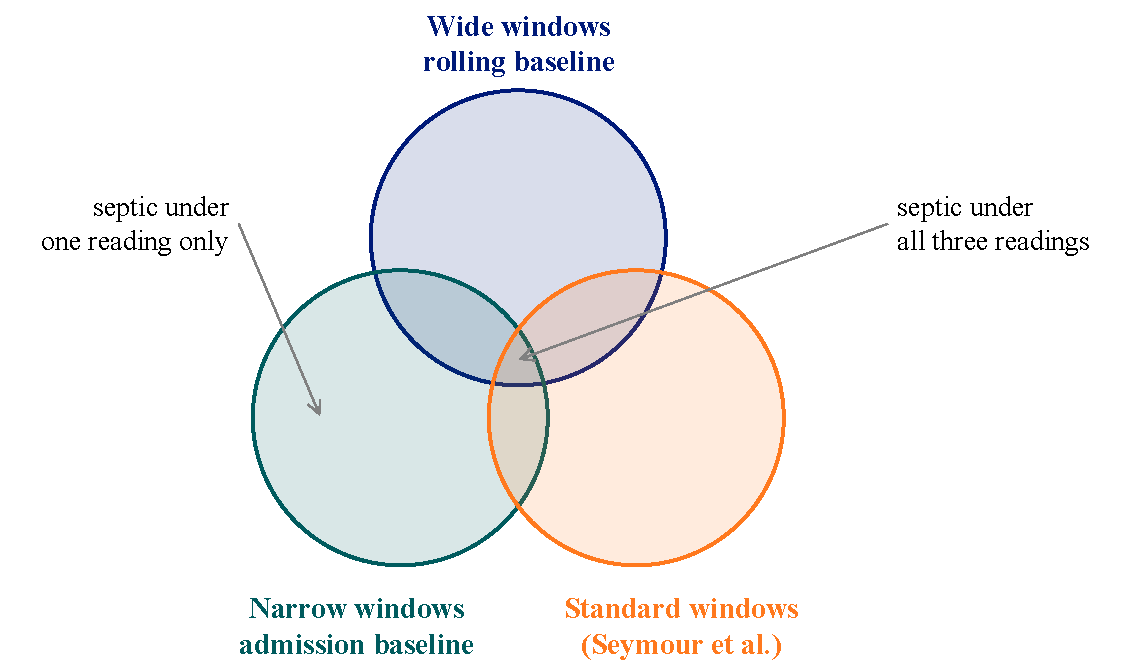
\includegraphics[width=0.92\textwidth]{figures-img/fig2.2_label_variance_concept.pdf}
    \caption{Schematic of label variation. Three defensible Sepsis-3
    interpretations applied to the same ICU population produce overlapping but
    distinct cohorts: only the central region is septic under all three
    readings, and each crescent holds patients counted by one reading alone.
    The corresponding MIMIC-IV measurement is reported in
    Chapter~\ref{ch:evaluation}, where the two narrowest readings agree at
    $\kappa = \pcKappaVsBA$.}
    \label{fig:label_variance_concept}
\end{figure}


\section{Clinical Actions in Sepsis Label Construction}
\label{sec:label_action}

Sepsis-3 defines sepsis as organ dysfunction in a patient with suspected
infection \cite{singer2016sepsis3}, and the operational criteria derived by
Seymour et al.\ \cite{seymour2016assessment} represent ``suspected infection''
through two clinician actions: drawing a culture and administering an
antibiotic. The operational label therefore depends partly on the timing of
clinician actions.

Kamran et al.\ \cite{kamran2024evaluation} examined this issue directly.
Clinicians frequently recognise and begin treating sepsis before the formal
criteria are met. A model trained to predict the moment the criteria are met is
therefore partly trained to predict \emph{when the clinician will act}, and the
physiological record available at prediction time is itself shaped by the
developing suspicion: tests are ordered, monitoring escalates, and observations
are recorded that would not otherwise exist. Re-evaluating the Epic Sepsis
Model on 77,582 hospitalisations, the authors report an AUROC of 0.62 when
predictions issued after clinical recognition are retained, falling to 0.47,
below chance, once they are excluded.

For a hazard model, a coefficient estimated on the interval up to Sepsis-3
onset therefore partly reflects clinician behaviour. Lactate measurement, for
example, may be prompted by clinical concern, creating dependence between the
predictor, clinical suspicion and the treatment-anchored outcome. Model
diagnostics such as proportional-hazards testing may not reveal this problem,
because it concerns outcome construction rather than statistical fit.
Addressing it requires an evaluation target that can precede the relevant
clinical actions.

Lauritsen et al.\ \cite{lauritsen2021framing} extend the problem beyond the
label to the surrounding design. They formalise \emph{framing} (the
observation window, the prediction window, the window shift, and the event that
triggers a prediction), enumerate eight possible framing structures, and
evaluate four on the same data. Framing affects both discrimination and
calibration and can produce opposing interpretations of the same physiological
variable: in their example, the apparent relationship of SpO$_2$ to sepsis
risk reverses direction with the framing. If framing can reverse the sign of a
coefficient, the coefficient reflects the study design as well as the patient.
Sign reversals are particularly consequential when coefficients are presented
as clinically interpretable effects, and H2 tests whether such instability
occurs on MIMIC-IV.

Treatment-anchored evaluation, as Kamran et al.\ apply it, restricts
\emph{when} performance is measured but leaves the treatment anchor inside the
label: a Sepsis-3 case is still a case only because a culture and an antibiotic
were ordered. SEP-1 and the CDC Adult Sepsis Event are also defined on
antibiotic days, so a comparison confined to these definitions cannot separate
definitional from empirical label variation. This motivates evaluating an
additional label that does not use treatment timestamps
(Section~\ref{sec:alt_labels}).


\section{Internal, Temporal and External Validation}
\label{sec:generalisation}

Table~\ref{tab:generalisation} summarises the published external-validation
record for real-time sepsis prediction.

\begin{table}[H]
    \centering\small
    \begin{tabularx}{\textwidth}{p{2.6cm}p{2.5cm}Xp{2.9cm}}
    \toprule
    \textbf{Study} & \textbf{Model} & \textbf{Transition} &
    \textbf{Degradation} \\
    \midrule
    Nemati et al.\ \cite{nemati2018aise} & Weibull--Cox (AISE) &
    Emory $\rightarrow$ MIMIC-III; AUROC 0.83--0.85 &
    Reported indistinguishable \\
    \addlinespace
    Reyna et al.\ \cite{reyna2020utility} & 853 Challenge entries &
    Two seen hospital systems $\rightarrow$ one unseen; rank correlation
    $\rho = 0.949$ between seen systems &
    $\rho = -0.033$ and $0.013$ to the unseen system \\
    \addlinespace
    Moor et al.\ \cite{moor2023review} & Deep temporal &
    Four international ICU databases, 136,478 admissions; internal AUC 0.846 &
    External AUC \textbf{0.761} ($-0.085$); 0.807 with 10\% fine-tuning \\
    \addlinespace
    Wang et al.\ \cite{wang2025srpm} & 91 models (meta-level) &
    Internal $\rightarrow$ external, full-window &
    AUROC $0.811 \rightarrow 0.783$ (n.s.); \textbf{Utility
    $0.381 \rightarrow -0.164$} \\
    \addlinespace
    Wong et al.\ \cite{wong2021epic} & Epic Sepsis Model v1 &
    Proprietary $\rightarrow$ Michigan Medicine, 38,455 hospitalisations &
    AUROC \textbf{0.63}; PPV 12\% \\
    \addlinespace
    Ostermayer et al.\ \cite{ostermayer2024external} & Epic Sepsis Model v1 &
    Proprietary $\rightarrow$ two county emergency departments &
    Sensitivity \textbf{14.7\%}; PPV 7.6\% \\
    \addlinespace
    Wong et al.\ \cite{wong2026epic} & Epic Sepsis Model v2 &
    Prospective, four US health systems, 227,091 encounters &
    AUROC 0.82--0.92 but \textbf{PPV 0.13--0.26}; 21--35 alerts per case \\
    \addlinespace
    Guo et al.\ \cite{guo2022temporal} & Feed-forward network &
    MIMIC-IV, within database, across admission eras &
    Sepsis \textbf{most degraded} of four tasks \\
    \bottomrule
    \end{tabularx}
    \caption{The published external-validation record for real-time sepsis
    prediction. Nemati et al.'s internal--external equivalence is the exception;
    their external set shares an era, a country and a care model with the
    development set, which is consistent with an external penalty that grows
    with the distance of the shift.}
    \label{tab:generalisation}
\end{table}

Across the studies summarised in Table~\ref{tab:generalisation}, three
patterns are relevant to this study.

\paragraph{One multi-database study reported an external AUROC reduction of
0.085.} Moor et al.\ report 0.846 $\rightarrow$ 0.761 across four databases
from the United States, the Netherlands and Switzerland, consistent in
direction, though not in significance, with Wang et al.'s meta-level 0.811
$\rightarrow$ 0.783. It is used here as a reference estimate for planning, not
as an established typical value. H5 asks whether the Utility Score declines
proportionally more than AUROC, so 0.085 bounds only the AUROC part of that
comparison.

\paragraph{Model rankings may not transfer across health systems.} Reyna et
al.\ report that team Utility Scores were strongly rank-correlated between the
two hospital systems on which participants trained ($\rho = 0.949$) but
essentially uncorrelated with performance on the third, unseen system
($\rho = -0.033$ and $0.013$). A published ranking therefore indicates little
about which model would perform best at a different hospital. Every comparator
in this study is refitted and rescored within the same pipeline, and published
figures are used only to bound expectations.

\paragraph{The split design is not neutral for sepsis.}
Guo et al.\ \cite{guo2022temporal} partitioned MIMIC-IV into four admission
eras (2008--2010, 2011--2013, 2014--2016, 2017--2019) and evaluated four
prediction tasks under temporal shift: mortality, long length of stay, sepsis
and invasive ventilation. Sepsis was the most affected. In that study, the
evaluated domain-generalisation and unsupervised domain-adaptation methods did
not consistently outperform empirical risk minimisation (AUROC differences
$-0.003$ to $0.050$). A random train/test split on MIMIC-IV may therefore give
an optimistic estimate for sepsis, more strongly than for the other ICU
outcomes evaluated. The primary validation uses a temporal split, and a random
split is retained to quantify any optimism (H4).

Dutta et al.\ \cite{dutta2026performance} did not detect temporal drift over
an 18-month prospective period within one health system, whereas Guo et al.\
examined shifts across a decade. The duration and context of the shift
therefore matter, and ``temporal validation'' is not a single practice.


\section{Discrimination versus Clinical Utility}
\label{sec:auroc_illusion}

A direct comparison is provided by Wang et al.\ \cite{wang2025srpm}. Across 91
models, the median AUROC moved from 0.811 internally to 0.783 externally, a
difference the authors report as not statistically significant, while the
median Utility Score moved from $+0.381$ to $-0.164$. For the same transition,
the two metrics disagree about whether performance changed.

The mechanism is well understood. AUROC is a ranking statistic, invariant to
monotone transformation of the score, so it cannot detect miscalibration, and
under low prevalence it is dominated by the large population of easily
classified true negatives. Across sites, the \emph{location} of the score
distribution relative to the alerting threshold tends to change more than the
\emph{ordering} of patients, and that location determines the false-alarm rate
and hence the utility. Van Calster et al.\ \cite{vancalster2019calibration}
identify calibration as a central weakness of predictive analytics for this
reason: a model that drives a threshold-based action depends on its
calibration whatever its AUROC.

Deployment results show the same pattern. The Epic Sepsis Model v2 combined
encounter-level AUROC of 0.82 to 0.92 with positive predictive value of 0.13 to
0.26 \cite{wong2026epic} (Table~\ref{tab:generalisation}), and Ostermayer et
al.\ \cite{ostermayer2024external}, validating version 1 independently in two
county emergency departments, report sensitivity of 14.7\% and PPV of 7.6\%.
Version 1 was a logistic regression and version 2 a gradient-boosted ensemble,
but version 2 also moved from global to local training, and Moor et al.\ show
that local fine-tuning alone recovers roughly half of the external penalty
($0.761 \rightarrow 0.807$). Model class and localisation therefore changed
together, and the comparison cannot isolate either effect.

Two benchmarks inform the evaluation plan. Moor et al.\ report their model
raising 1.4 false alerts per true alert while detecting 80\% of septic
patients a median of 3.7 hours (95\% CI 3.0--4.3) before onset. This provides a
reference for alert burden and a realistic lead time for a modern system, in
contrast to the 28 hours of the original TREWScore headline
\cite{henry2015trewscore}. Seymour et al.\ \cite{seymour2017time}, across
49,331 patients at 149 New York hospitals, estimate an odds ratio for
in-hospital mortality of 1.04 per additional hour before antibiotic
administration. The clinical value of a lead time of a few hours therefore
depends on the alert being acted on, on the patient not otherwise being
recognised in time, and on the cost of the false alerts.

These findings indicate that evaluation should include calibration, AUPRC,
utility or net benefit, and alert burden in addition to AUROC, and these
measures are central to this study's evaluation. The adapted Utility Score is
the primary clinical metric, while AUROC is the metric on which the
pre-registered comparative hypotheses are stated. Because the utility metric
is threshold-dependent, it is reported across a swept grid of operating points
(Section~\ref{sec:clinical_utility}).


\section{Methodological Challenges in Survival Modelling}
\label{sec:survival_dispute}

Dynamic ICU prediction raises several methodological issues for conventional
survival models.

\begin{enumerate}
    \item \textbf{Proportional hazards may fail in sepsis cohorts.}
    Kasal et al.\ \cite{kasal2004cox} compared a standard Cox model with
    Gray's flexible survival model in a large severe-sepsis cohort and found
    hazards for death after sepsis frequently non-proportional. The assumption
    is often untested in MIMIC work.

    \item \textbf{Independent censoring may also fail.} Resche-Rigon et al.\
    \cite{rescherigon2006competing} argue that discharge alive is not a
    non-informative censoring event in ICU cohorts: patients discharged alive
    are systematically unlike those who remain, so the assumption underlying
    Kaplan--Meier estimation is violated. Fine--Gray subdistribution hazard
    modelling \cite{finegray1999subdistribution} is one common approach to
    competing risks.

    \item \textbf{Competing-risks methods are themselves contested.} Schoenfeld
    \cite{schoenfeld2006survival} argues that survival methods, explicitly
    including competing-risks methods, are inappropriate for ICU outcome
    studies, and that studies seeking prognostic covariates should use logistic
    regression instead.

    \item \textbf{Landmarking does not restore proportional hazards.}
    Landmarking, which refits the model at each prediction time on the subset
    still at risk, provides one practical approach to updating predictions over
    time \cite{vanhouwelingen2007landmark}. It does not in general satisfy the
    proportional-hazards assumption; it is a different model with its own
    approximation error.

    \item \textbf{Joint models are rigorous but computationally costly.}
    Modelling longitudinal biomarker trajectories and the event process through
    shared latent structure outperforms landmarking when the longitudinal
    sub-model is correctly specified \cite{rizopoulos2017joint}, but the
    approach is computationally expensive, requires a common baseline time, and
    scales poorly to the heterogeneous, irregularly sampled, high-dimensional
    streams of an ICU record.
\end{enumerate}

This study adopts a \textbf{discrete-time hazard model}, fitted as a pooled
logistic regression over person-hour records with time-varying covariates and
a flexible baseline hazard. Pooled logistic regression approximates
time-dependent Cox regression when intervals are short and interval-specific
event probabilities are low \cite{dagostino1990pooled}, and Ngwa et al.\
\cite{ngwa2016comparison} confirmed the close agreement by simulation. The
hourly intervals and low observed event rates place this application within
the setting in which the approximation is expected to be close.

The formulation addresses the issues above as follows. It does not assume
proportional hazards (item~1). A multinomial cause-specific formulation over
the person-hour models discharge alive and death without sepsis as distinct
competing outcomes \cite{rescherigon2006competing, heyard2019dynamic}
(item~2). It retains a logistic-regression likelihood while modelling time
explicitly (item~3). Its output is an hourly risk score, the object the
Challenge utility metric consumes, so it is directly comparable with the
machine-learning literature. Heyard et al.\ \cite{heyard2019dynamic,
heyard2020evaluation} supply development and validation methodology for
discrete time-to-event data with competing risks, and
Chapter~\ref{ch:methodology} gives the full specification.

A conventional Cox model is retained as a benchmark to quantify the effect of
the proportional-hazards and censoring assumptions, and its Schoenfeld test is
reported.


\section{Choice of Rule-Based Comparator}
\label{sec:comparator_choice}

Most MIMIC-IV sepsis models benchmark against SIRS, qSOFA and NEWS. Two results
constrain how that benchmark should be read.

The Surviving Sepsis Campaign guidelines \cite{evans2021ssc} issue a strong
recommendation \emph{against} using qSOFA as a sole screening tool, citing poor
sensitivity, so superiority over qSOFA is a weak claim. The National Early
Warning Score 2 (NEWS2), which aggregates six physiological parameters
(respiratory rate, oxygen saturation, systolic blood pressure, pulse rate,
level of consciousness and temperature) into a bedside deterioration score, is
therefore used as the principal rule-based comparator, with qSOFA and SIRS
reported for completeness.

Mellhammar et al.\ \cite{mellhammar2020news2} provide a direct precedent. They
derived a score using LASSO on prospectively collected emergency-department
data and validated it against NEWS2 and RETTS; the derived score did not
outperform NEWS2 (AUC 0.73 versus 0.69, $p = 0.32$), and the authors concluded
that a statistical approach did not yield better sepsis risk stratification
than NEWS2. The aim here is therefore not to derive a deployable score but to
compare model classes against a clinically used benchmark.


\section{Equity and Subgroup Validity}
\label{sec:equity_lit}

Wang, Li, Naidech and Luo \cite{wang2022equity} was the only directly relevant
source on subgroup validity in a MIMIC sepsis cohort identified in the search.
The study analysed 11,791 MIMIC-III critical-care patients, of whom 5,783 met
Sepsis-3 criteria, and reports two findings. First, six competing sepsis
identification criteria selected systematically different sub-populations with
respect to race, marital status, insurance type and language, so
classification as septic in MIMIC is not demographically neutral. Second,
\textbf{mortality} prediction among patients already identified as septic
degraded significantly when a model trained on the full population was applied
to Asian, Hispanic and Spanish-speaking patients, with pairwise testing
detecting significant discrepancies between Asian and White patients and
between English- and Spanish-speaking patients.

Because the second finding concerns mortality rather than onset, it does not
provide a prior estimate for an onset model's subgroup discrimination, and the
two findings concern different targets and cannot be compared directly. They
nevertheless show that the label is differentially sensitive by subgroup and
that model performance can differ across overlapping subgroups. These findings
support treating subgroup analysis as part of model validity assessment, and
connect it to the label problem of Section~\ref{sec:label_object};
Chapter~\ref{ch:methodology} describes how both quantities are measured here.

A methodological caution from the same source governs how the results in
Section~\ref{sec:equity} are read. MIMIC's demographic fields are
administrative records, not measured population attributes. The race field
mixes broad categories with more granular ones drawn from the same population,
and includes values that record the absence of an answer rather than an
answer. Subgroup contrasts computed on such a field compare administrative
strata and are interpreted in those terms.


\section{Interpretability and Label Uncertainty}
\label{sec:interpretability_survives}

The main advantage of a coefficient-based hazard model in this setting is not
necessarily higher performance but transparent assumptions and interpretable
coefficients, and Christodoulou et al.\ \cite{christodoulou2019cox} suggest
that little discrimination is sacrificed for them. Cohen et al.\
\cite{cohen2024subtle} and Lauritsen et al.\ \cite{lauritsen2021framing}
qualify that advantage: if the identified cohort varies by a factor of 2.5
with the onset rule, and framing can reverse the sign of an estimated
association, a coefficient reported without a label-sensitivity analysis
reflects both biology and the recording process.

Coefficient interpretation therefore depends on a stable and clearly defined
outcome. Stability across plausible label definitions strengthens the case for
interpreting a coefficient, whereas sign reversal indicates sensitivity to
outcome construction. The search identified no such analysis for a survival
model on MIMIC-IV.

The problems reviewed in this chapter (label variation, the label's dependence
on clinical action, split design and metric choice) have each been
demonstrated separately, by different groups using different databases and
models. The evidence therefore motivates estimating the effects of label,
prediction timing, split, metric and model choices within a common dataset and
pipeline, which is the research question of Section~\ref{sec:rq}.


\section{Summary: Design Decisions and Their Evidence}
\label{sec:design_warrant}

Table~\ref{tab:design_warrant} maps each major design decision to the evidence
supporting it.

{\small
\begin{longtable}{p{3.1cm}p{5.6cm}p{4cm}}
    \caption{Design decisions and supporting evidence.}\label{tab:design_warrant}\\
    \toprule
    \textbf{Decision} & \textbf{Reason} & \textbf{Source} \\
    \midrule
    \endfirsthead
    \toprule
    \textbf{Decision} & \textbf{Reason} & \textbf{Source} \\
    \midrule
    \endhead
    \bottomrule
    \endfoot

        Three label variants & Label- and model-related AUROC ranges of
        similar magnitude were reported &
        Cohen et al.\ \cite{cohen2024subtle} \\
        Label as a studied factor & Label sensitivity was replicated
        prospectively at scale &
        Cohen; Dutta et al.\ \cite{dutta2026performance} \\
        Discrete-time model & Pooled logistic regression approximates
        time-dependent Cox regression at short intervals, without a
        proportional-hazards assumption &
        D'Agostino \cite{dagostino1990pooled};
        Ngwa \cite{ngwa2016comparison};
        Schoenfeld \cite{schoenfeld2006survival} \\
        Competing risks & Discharge alive is informative rather than
        non-informative censoring &
        Resche-Rigon \cite{rescherigon2006competing};
        Heyard \cite{heyard2019dynamic} \\
        Cox benchmark & Proportional hazards may fail in sepsis cohorts &
        Kasal et al.\ \cite{kasal2004cox} \\
        No case--control matching & Control alignment can inflate apparent
        performance &
        Moor et al.\ \cite{moor2021review} \\
        Treatment-anchored evaluation & Models may learn clinician suspicion
        rather than deterioration &
        Kamran et al.\ \cite{kamran2024evaluation} \\
        Anchor-independent label & Sepsis-3, SEP-1 and CDC ASE all depend on
        treatment timing &
        Kamran \cite{kamran2024evaluation};
        Dutta \cite{dutta2026performance} \\
        Temporal split primary & Sepsis was the most affected of four MIMIC-IV
        tasks under temporal shift &
        Guo et al.\ \cite{guo2022temporal} \\
        Comparators refitted in-pipeline & Published rankings may not transfer
        across hospital systems &
        Reyna et al.\ \cite{reyna2020utility} \\
        Utility Score primary & AUROC may change little despite a substantial
        decline in utility &
        Wang et al.\ \cite{wang2025srpm} \\
        Utility swept, not fixed & A threshold-dependent metric at one cut-off
        can be dominated by calibration and threshold selection &
        Reyna \cite{reyna2020utility};
        Wong \cite{wong2026epic} \\
        Calibration co-primary & Threshold-based decisions depend on
        calibration whatever the AUROC &
        Van Calster et al.\ \cite{vancalster2019calibration} \\
        Alert burden reported & A multi-database deep model reported 1.4 false
        alerts per true alert &
        Moor et al.\ \cite{moor2023review} \\
        NEWS2 as principal benchmark & qSOFA is not recommended as a sole
        screening tool, and a LASSO-derived score did not outperform NEWS2 &
        Evans \cite{evans2021ssc};
        Mellhammar \cite{mellhammar2020news2} \\
        GBT comparator & Model-class equivalence is supported for tabular
        prediction but contested for temporal early warning &
        Christodoulou \cite{christodoulou2019cox};
        Fagerstr{\"o}m \cite{fagerstrom2019lisep} \\
        Subgroup label sensitivity & Label composition varies demographically,
        and no onset-model subgroup discrimination study was identified &
        Wang et al.\ \cite{wang2022equity} \\
        TRIPOD+AI / PROBAST+AI & The reporting standards cover regression and
        machine learning under one checklist &
        Collins \cite{collins2024tripodai};
        Moons \cite{moons2025probastai} \\
\end{longtable}
}
